\documentclass[11pt,a4paper]{article}

%========== PACKAGES ==========%

\usepackage{a4wide} 			% save some rainforests
\usepackage{amsmath,amssymb}	% for mathematical notation
\usepackage[english]{babel}		% language definition
\usepackage{color}				% to make syntax pretty
\usepackage{enumerate}			% roman enumeration
\usepackage{fancyref}			% fancy references
\usepackage{float}				% for precise placement
\usepackage{graphicx}			% importing graphics
\usepackage[utf8]{inputenc} 	% can we has UTF-8, plox
\usepackage{listings}			% code listings
\usepackage{multicol} 			% for column layout
\usepackage{multirow}			% ...
\usepackage{tikz}				% pretty drawings

%========== DEFINITIONS ==========%

\definecolor{comment}{rgb}		{0.38, 0.62, 0.38}
\definecolor{keyword}{rgb}		{0.10, 0.10, 0.81}
\definecolor{identifier}{rgb}	{0.00, 0.00, 0.00}
\definecolor{string}{rgb}		{0.50, 0.50, 0.50}

\let\imp\to

\newcommand{\specialcell}[2][l]{%
\begin{tabular}[#1]{@{}l@{}}#2\end{tabular}}

%========== SETTINGS ==========%

\lstset
{
	% general settings
	numbers=left,
	frame=single,
	basicstyle=\footnotesize\ttfamily,
	tabsize=2,
	% syntax highlighting
	commentstyle=\color{comment},
	keywordstyle=\color{keyword},
	identifierstyle=\color{identifier},
	stringstyle=\color{string},
}

%========== DECLARATIONS ==========%

\title
{
	\vspace{-1in}
	{\large Individual Assignment 5}\\
	Compilers
}

\author
{
	Casper B. Hansen\\
	Department of Computer Science\\
	University of Copenhagen\\
	{\tt fvx507@alumni.ku.dk}
}

%========== DOCUMENT ==========%

\begin{document}

\clearpage
\maketitle

\section{Exercise 1}
Given the following program:
\begin{lstlisting}
gcd(a,b) [
	LABEL start
	IF a < b THEN next ELSE swap
	LABEL swap
	t := a
	a := b
	b := t
	LABEL next
	z := 0
	b := b mod a
	IF b = z THEN end ELSE start
	LABEL end
	RETURN a
]
\end{lstlisting}

\subsection*{a \mdseries Show {\bf succ}, {\bf gen} and {\bf kill} sets for
every instruction in the program.}
\begin{figure}[H]
	\center

	\begin{multicols}{2}

	\begin{tabular}{|c|c|c|c|}
		\hline
		{\bf i}	& {\bf succ[i]}	& {\bf gen[i]}	& {\bf kill[i]} \\ \hline
		1	& $\{2\}$		& $\{a,b\}$		& $\emptyset$	\\ \hline
		2	& $\{3\}$		& $\emptyset$	& $\emptyset$	\\ \hline
		3	& $\{4,8\}$		& $\{a,b\}$		& $\emptyset$	\\ \hline
		4	& $\{5\}$		& $\emptyset$	& $\emptyset$	\\ \hline
		5	& $\{6\}$		& $\{a\}$		& $\{t\}$ 		\\ \hline
		6	& $\{7\}$		& $\{b\}$		& $\{a\}$		\\ \hline
		7	& $\{8\}$		& $\{t\}$		& $\{b\}$		\\ \hline
	\end{tabular}

	\vfill
	\columnbreak

	\begin{tabular}{|c|c|c|c|}
		\hline
		{\bf i}	& {\bf succ[i]}	& {\bf gen[i]}	& {\bf kill[i]} \\ \hline
		8	& $\{9\}$		& $\emptyset$	& $\emptyset$	\\ \hline
		9	& $\{10\}$		& $\emptyset$	& $\{z\}$		\\ \hline
		10	& $\{11\}$		& $\{a,b\}$		& $\{b\}$		\\ \hline
		11	& $\{2,12\}$	& $\{b,z\}$		& $\emptyset$	\\ \hline
		12	& $\{13\}$		& $\emptyset$	& $\emptyset$	\\ \hline
		13	& $\emptyset$	& $\{a\}$		& $\emptyset$	\\ \hline
	\end{tabular}

	\end{multicols}

	\label{fig:sets}
	\caption{{\bf succ}, {\bf gen} and {\bf kill} sets}

\end{figure}

\newpage
\subsection*{b \mdseries Compute {\bf in} and {\bf out} sets for every
instruction, show the fix-point iteration.}
Following the set equations
\begin{align}
	\text{\bf in[$i$]}
	&= \text{\bf gen[$i$]} \cup
	(\text{\bf out[$i$]}{\ }\backslash{\ }\text{\bf kill[$i$]} ) \\
	\text{\bf out[$i$]}
	&= \bigcup_{j \in \text{\bf succ[$i$]}}^n \text{\bf in[$j$]}
\end{align}
we perform the fixed-point iterations
\begin{figure}[H]

	\center
	\begin{multicols}{3}

		{\bf Initial} \\\vspace{0.10in}
		\begin{tabular}{|c||c|c|}
			\hline
			{\bf i}		& {\bf out[i]}		& {\bf in[i]}	\\ \hline
			{\bf 1}		& $\emptyset$		& $\emptyset$	\\ \hline
			{\bf 2}		& $\emptyset$		& $\emptyset$	\\ \hline
			{\bf 3}		& $\emptyset$		& $\emptyset$	\\ \hline
			{\bf 4}		& $\emptyset$		& $\emptyset$	\\ \hline
			{\bf 5}		& $\emptyset$		& $\emptyset$	\\ \hline
			{\bf 6}		& $\emptyset$		& $\emptyset$	\\ \hline
			{\bf 7}		& $\emptyset$		& $\emptyset$	\\ \hline
			{\bf 8}		& $\emptyset$		& $\emptyset$	\\ \hline
			{\bf 9}		& $\emptyset$		& $\emptyset$	\\ \hline
			{\bf 10}	& $\emptyset$		& $\emptyset$	\\ \hline
			{\bf 11}	& $\emptyset$		& $\emptyset$	\\ \hline
			{\bf 12}	& $\emptyset$		& $\emptyset$	\\ \hline
			{\bf 13}	& $\emptyset$		& $\emptyset$	\\ \hline
		\end{tabular}

		\vfill
		\columnbreak
			
		{\bf 1st iteration} \\\vspace{0.10in}
		\begin{tabular}{|c||c|c|}
			\hline
			{\bf i}		& {\bf out[i]}		& {\bf in[i]}	\\ \hline
			{\bf 1}		& $\{a,b\}$			& $\{a,b\}$		\\ \hline
			{\bf 2}		& $\{a,b\}$			& $\{a,b\}$		\\ \hline
			{\bf 3}		& $\{a,b\}$			& $\{a,b\}$		\\ \hline	% + 8
			{\bf 4}		& $\{a,b\}$			& $\{a,b\}$		\\ \hline
			{\bf 5}		& $\{b,t\}$			& $\{a,b\}$		\\ \hline	% t
			{\bf 6}		& $\{a,t\}$			& $\{b,t\}$		\\ \hline	% a
			{\bf 7}		& $\{a,b\}$			& $\{a,t\}$		\\ \hline	% b
			{\bf 8}		& $\{a,b\}$			& $\{a,b\}$		\\ \hline
			{\bf 9}		& $\{a,b,z\}$		& $\{a,b\}$		\\ \hline	% z
			{\bf 10}	& $\{a,b,z\}$		& $\{a,b,z\}$	\\ \hline
			{\bf 11}	& $\{a\}$			& $\{a,b,z\}$	\\ \hline	% + 2
			{\bf 12}	& $\{a\}$			& $\{a\}$		\\ \hline
			{\bf 13}	& $\{a\}$			& $\{a\}$		\\ \hline
		\end{tabular}

		\vfill
		\columnbreak

		{\bf 2nd iteration} \\\vspace{0.10in}
		\begin{tabular}{|c||c|c|}
			\hline
			{\bf i}		& {\bf out[i]}		& {\bf in[i]}	\\ \hline
			{\bf 1}		& $\{a,b\}$			& $\{a,b\}$		\\ \hline
			{\bf 2}		& $\{a,b\}$			& $\{a,b\}$		\\ \hline
			{\bf 3}		& $\{a,b\}$			& $\{a,b\}$		\\ \hline	% + 8
			{\bf 4}		& $\{a,b\}$			& $\{a,b\}$		\\ \hline
			{\bf 5}		& $\{b,t\}$			& $\{a,b\}$		\\ \hline	% t
			{\bf 6}		& $\{a,t\}$			& $\{b,t\}$		\\ \hline	% a
			{\bf 7}		& $\{a,b\}$			& $\{a,t\}$		\\ \hline	% b
			{\bf 8}		& $\{a,b\}$			& $\{a,b\}$		\\ \hline
			{\bf 9}		& $\{a,b,z\}$		& $\{a,b\}$		\\ \hline	% z
			{\bf 10}	& $\{a,b,z\}$		& $\{a,b,z\}$	\\ \hline
			{\bf 11}	& $\{a\}$			& $\{a,b,z\}$	\\ \hline	% + 2
			{\bf 12}	& $\{a\}$			& $\{a\}$		\\ \hline
			{\bf 13}	& $\{a\}$			& $\{a\}$		\\ \hline
		\end{tabular}

	\end{multicols}

	\label{fig:fixed-point-iterations}
	\caption{First fixed-point iterations}

\end{figure}

\subsection*{c \mdseries Draw the interference graph for {\tt a}, {\tt b},
{\tt t}, and {\tt z}.}
Firstly, we give a table showing the interference
\begin{figure}[H]

	\center
	\begin{tabular}{|c||c|c|}
		\hline
		{\bf Instruction}	& {\bf Left-hand side}	& {\bf Right-hand side}	\\ \hline
		5					& $\{t\}$				& $\{b\}$				\\ \hline
		6					& $\{a\}$				& $\{t\}$				\\ \hline
		7					& $\{b\}$				& $\{a\}$				\\ \hline
		9					& $\{z\}$				& $\{a,b\}$				\\ \hline
		10					& $\{b\}$				& $\{a,z\}$				\\ \hline
	\end{tabular}

	\label{fig:interference-table}
	\caption{Interference table}

\end{figure}
\newpage
Now that we have determined which variables that interferes with one another
we can produce the interference graph.
\begin{figure}[H]

	\center
	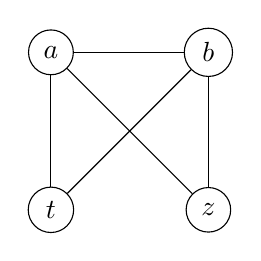
\begin{tikzpicture}
	[
		scale=1.00,
		node/.style = {circle, align=center, draw=black, fill=none},
	]

	% times symbols
	\node[node] (a) 	at ( -1.0,  1.0 ) {$a$};
	\node[node] (b) 	at (  1.0,  1.0 ) {$b$};
	\node[node] (t) 	at ( -1.0, -1.0 ) {$t$};
	\node[node] (z) 	at (  1.0, -1.0 ) {$z$};

	\foreach \from/\to in {a/t,b/a,b/z,t/b,z/a,z/b}
	\draw[solid] (\from) -- (\to);

	\end{tikzpicture}

	\label{fig:interference-graph}
	\caption{Interference graph}

\end{figure}

\subsection*{d \mdseries Color the interference graph with 3 colors. Show the
stack.}
We will now color code every vertex in the graph, each color representing an
available register.

Since $t$ and $z$ aren't connected by an edge, we let those variables share a
color
\begin{multicols}{2}

	\begin{figure}[H]

		\center
		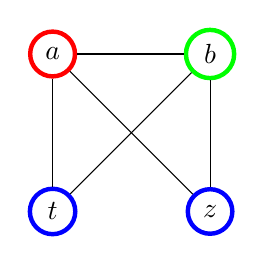
\begin{tikzpicture}
		[
			scale=1.00,
			node/.style = {circle, align=center, draw=black, fill=none},
			rnode/.style = {circle, align=center, draw=red, fill=none},
			gnode/.style = {circle, align=center, draw=green, fill=none},
			bnode/.style = {circle, align=center, draw=blue, fill=none},
		]

		% times symbols
		\node[ultra thick, rnode] (a) 	at ( -1.0,  1.0 ) {$a$};
		\node[ultra thick, gnode] (b) 	at (  1.0,  1.0 ) {$b$};
		\node[ultra thick, bnode] (t) 	at ( -1.0, -1.0 ) {$t$};
		\node[ultra thick, bnode] (z) 	at (  1.0, -1.0 ) {$z$};

		\foreach \from/\to in {a/t,b/a,b/z,t/b,z/a,z/b}
		\draw[solid] (\from) -- (\to);

		\end{tikzpicture}

		\label{fig:3-color-interference-graph}
		\caption{3-color interference graph}

	\end{figure}

	\vfill
	\columnbreak

	\begin{figure}[H]

		\center
		\begin{tabular}{|c|c|c|}
			\hline
			{\bf Node}	& {\bf Neighbors}	& {\bf Color} \\ \hline
			$a$			& $\emptyset$		& {\color{red} 1} \\ \hline
			$b$			& $\{a\}$			& {\color{green} 2} \\ \hline
			$t$			& $\{a,b\}$			& {\color{blue} 3} \\ \hline
			$z$			& $\{a,b\}$			& {\color{blue} 3} \\ \hline
		\end{tabular}

		\label{fig:interference-table}
		\caption{Interference table}

	\end{figure}

\end{multicols}

\subsection*{e \mdseries Color the interference graph with 2 colors. Select
variables to spill, perform the spilling transformation and show the resulted
program (with allocated registers and spilling).}
Following the n-coloring algorithm with $n = 2$, we get the following
interference graph and stack.
\begin{multicols}{2}

	\begin{figure}[H]

		\center
		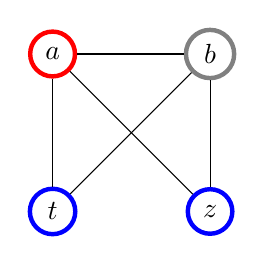
\begin{tikzpicture}
		[
			scale=1.00,
			node/.style = {circle, align=center, draw=gray, fill=none},
			rnode/.style = {circle, align=center, draw=red, fill=none},
			bnode/.style = {circle, align=center, draw=blue, fill=none},
		]

		% times symbols
		\node[ultra thick, rnode] (a) 	at ( -1.0,  1.0 ) {$a$};
		\node[ultra thick, node] (b) 	at (  1.0,  1.0 ) {$b$};
		\node[ultra thick, bnode] (t) 	at ( -1.0, -1.0 ) {$t$};
		\node[ultra thick, bnode] (z) 	at (  1.0, -1.0 ) {$z$};

		\foreach \from/\to in {a/t,b/a,b/z,t/b,z/a,z/b}
		\draw[solid] (\from) -- (\to);

		\end{tikzpicture}

		\label{fig:2-color-interference-graph}
		\caption{2-color interference graph}

	\end{figure}

	\vfill
	\columnbreak

	\begin{figure}[H]

		\center
		\begin{tabular}{|c|c|c|}
			\hline
			{\bf Node}	& {\bf Neighbors}	& {\bf Color}			\\ \hline
			$a$			& $\emptyset$		& {\color{red}		1}	\\ \hline
			$t$			& $\{a\}$			& {\color{blue}		2}	\\ \hline
			$b$			& $\{a,t\}$			& spilled				\\ \hline
			$z$			& $\{a,b\}$			& {\color{blue}		2}	\\ \hline
		\end{tabular}

		\label{fig:interference graph}
		\caption{Interference graph}

	\end{figure}

\end{multicols}
\newpage
Having decided which variables need to be spilled, we can now alter the
original program to reflect this.
\begin{lstlisting}[mathescape]
gcd(a,b) [
	b := M[address$_b$]
	LABEL start
	b$_5$ := M[address$_b$]
	IF a < b$_5$ THEN next ELSE swap
	LABEL swap
	t := a
	b$_9$ := M[address$_b$]
	a := b$_9$
	b$_{10}$ := t
	M[address$_b$] := b$_{10}$
	LABEL next
	z := 0
	b$_{15}$ := M[address$_b$]
	b$_{15}$ := b$_{15}$ mod a
	M[address$_b$] := b$_{15}$
	b$_{18}$ := M[address$_b$]
	IF b$_{18}$ = z THEN end ELSE start
	LABEL end
	RETURN a
]
\end{lstlisting}

\newpage
\section{Exercise 2}
% refers to Intermediate Code Generation Slides / Book Chapter.
Introduce two more statements to the source language:
\begin{align*}
	\text{\tt Stat} \rightarrow \text{\tt break}
	\qquad
	\text{\tt Stat} \rightarrow \text{\tt continue}
\end{align*}
where {\tt break} and {\tt continue} are assumed to appear only inside loops,
be them {\tt while} or {\tt repeat-until} loops. They have  the following
semantics (similar to C/Java):
\begin{enumerate}
	\item {\tt break} jumps immediately after the loop
	\item {\tt continue} jumps to a label just before where the loop condition
	is tested
\end{enumerate}
Your tasks is to translate these newly introduced statements (and their
semantics) to the lecture's three-address intermediate code (IL).

This probably also requires modifications to function {\tt TransStat}, e.g.,
extra parameters, and extending the implementation of {\tt while}-loop and
{\tt repeat-until} loop statements.

% HINT:	a loop creates two new labels, one placed just before testing the
%		loop condition (target of continue), the other placed just after the
%		loop (target of break).  These two labels (options) are passed as
%		parameters to TransStat.

\subsection*{Solution}
Following the advice of the assignment, we need to add two extra parameters to
{\tt Trans$_{Stat}$}, namely {\tt label$_b$} and {\tt label$_c$}. Their
contents are the labels to jump to for {\tt break} and {\tt continue},
respective.

This allows us to use these labels when we encounter the two keywords, as
shown below.
\begin{figure}[H]
	
	\text{\tt Trans$_{Stat}$(stat, label$_b$, label$_c$, vtable, ftable)
	= case of stat} \\
	\begin{tabular}{ll}
		\hline
		\tt break & \tt [GOTO label$_b$] \\ \hline
		\tt continue & \tt [GOTO label$_c$] \\ \hline
	\end{tabular}

\end{figure}
Note that, since the keywords {\tt break} and {\tt continue} are specialized
for use only within loops, we must throw a compiler error should we encounter
either of these outside a loop. This could theoretically simply be done by
passing a {\tt NULL}-value for these in statements that do no have an outer
loop (eg. an if-then-else statement), otherwise the labels are inherited from
the previous statement allowing escape from deeper scopes. I would, however,
assume that the best place to handle such an error, would be at the parsing
stage.

Now, inside of the {\tt repeat-until}- and {\tt while}-loops we replace the
line
\begin{align*}
	\text{\tt code$_n$ = Trans$_{Stat}$(stat, vtable, ftable)}
\end{align*}
\begin{center}with\end{center} \vspace{-0.12in}
\begin{align*}
	\text{\tt code$_n$ = Trans$_{Stat}$(stat, label$_b$, label$_c$, vtable, ftable)}
\end{align*}
Where {\tt label$_b$} is the appropriate label for {\tt break} (i.e.
{\tt label$_t$} in case of {\tt repeat-until} and {\tt label$_f$} in case of
{\tt while}). Likewise, {\tt label$_c$} is the appropriate label for
{\tt continue} (i.e. {\tt label$_f$} in case of {\tt repeat-until} and
{\tt label$_s$} in case of {\tt while}). Any other statement should simply
pass on the label arguments, so they can be reached from deeper scopes (ie. an
if-statement). 

This effectively allows regular statements inside of loops, but limits
loop-specific statements to reside only within loops.

\end{document}
